\documentclass[a4paper,12pt, titlepage]{article}
%\usepackage{color}
%\definecolor{light-gray}{gray}{0.95}

\usepackage{xcolor}
\usepackage{alltt}
\usepackage{url}
\usepackage{tikz}
\usetikzlibrary{trees}

\definecolor{light-gray}{gray}{0.95}
% Compensate for fbox sep:
\newcommand\Hi[2][light-gray]{%
  \hspace*{-\fboxsep}%
  \colorbox{#1}{#2}%
  \hspace*{-\fboxsep}%
}

		% This is my own macro !!!

\title{Issuer Control}


	
\begin{document}
\maketitle

\section{System work-flow}
The idea is to build the system in a generic way such that the interface can be described in XML and built at runtime. This means that if (when) the Cronos API / issuer setup changes the code does not need to be modified. If the system had to be modified every-time something in Cronos changed or the steps involved in issuer setup changed it would quickly become unmaintained and unused. Below I have outlined a possible solution below but the basic functional requirements are as follows.
\begin{itemize}
\item Request specification; The request must be specified using some kind of markup that will allow the following information for each parameter \label{section:required metadata}
	\begin{itemize}
	\item Type
	\item Required, optional or hidden
	\item Default values
	\item UI component (ex, ComboBox, TextField, List etc) Might be best to imply this from type and default values but still be able to specify it if needed.
	\end{itemize}
\item Request flow specification; The work flow for the wizard should consist of a number of steps, each containing requests.
\item Submit requests; Again, need to be done generically. Easiest way is probably dynamic class invocation at runtime.
\end{itemize}
\section{Possible implementation}
	\subsection{Request specification using XSD}
	Specify requests in XML. The requests specification could be done by using the existing XSD for Cronos and annotating it with default values. Information such as type (already in Oil to some degree) and required / optional use is already contained within the schema and can be easily changed. Important to know that the requests are not built from the XSD, they are built with oil objects as normal, the XSDs are use to generate the UI and map the various fields to the correct parameters in the corresponding Oil object.
	\begin{verbatim}
<xsd:complexType mixed="true" name="GetVCNServiceStatusResponseType">
    <xsd:attribute name="Enabled" type="xsd:boolean" use="optional"/>
    <xsd:attribute name="RequestId" type="xsd:string" use="optional"/>
    <xsd:attribute name="Pan" type="PanConstraintType" use="optional"/>
    <xsd:attribute name="CpnId" type="xsd:decimal" use="optional"/>
</xsd:complexType>
	\end{verbatim}
	An XSD allows constraints to be specified which could be used to populate combo-boxs / lists, or used as default values in text fields (in this case the constraint would be ignored and just used to specify a default value). This does add an additional layer to the parser.
	\begin{verbatim}
<xsd:simpleType name="VelocityPeriodConstraintType">
    <xsd:restriction base="xsd:string">
    <xsd:enumeration value="D"/>
    <xsd:enumeration value="W"/>
    <xsd:enumeration value="Q"/>
    <xsd:enumeration value="C"/>
    <xsd:enumeration value="M"/>
    <xsd:enumeration value="Y"/>
    </xsd:restriction>
</xsd:simpleType>
	\end{verbatim}
		\subsubsection{Positives}
		\begin{itemize}
		\item Schemas are already created and can be automatically regenerated every time a request changes using schema server.
		\item Allows system to be easily modified to reflect changes to Cronos / issuer setup. No code changes to completely change the UI and underlying requests
		\end{itemize}
		\subsubsection{Negatives}
		\begin{itemize}
		\item Existing XSD parsers (JAXB) seem to be mainly concerned with generating classes from and XSD (the operate like a code generator). Oil already does this, we just want to populate the Oil objects with values. Needs further investigation, but will probably have to parse the XSDs like plain old XML
		\item Schemas may require a lot of annotation. If this has to be done each time a new schema is generated it would defeat the purpose of using the schemas.
		\item When changes to Cronos are made the XSD must be generated and copied into the project. This could be automated fairly easily (I think).
		\end{itemize}
	\subsection{Request specification using Oil}
Request specification is done using the Oil objects. An OilBean is a hashmap; the key set can be used to build a request UI. Each member in the OilBean members map contains some limited metadata. The only really useful thing here is the type, Number or String. An additional file containing the metadata described above would be needed.
	\begin{verbatim}
<Request Name="SetIssuerSMSProperties">
    <Param Name="id" Type="string" Use="required"/>
    <Param Name="shortcode" type="number" Use="optional" uiElem="JComboBox">
        <Defaults>
            <Value>12345</Value>
            <Value>56789</Value>
        <Defaults>
    </Parm>
</Request>

	\end{verbatim}

		\subsubsection{Positives}
		\begin{itemize}
		\item Using the OilBeans to specify the requests cuts down on a lot of the markup needed in the first approach. Additionally, to update the wizard when changes to Cronos are made it just needs to be tagged and built.
		\item Separation of request specification and metadata allows requests to change without any modification of XML unless needed.
		\end{itemize}
		\subsubsection{Negatives}
		\begin{itemize}
		\item Separation of request specification and metadata can make it hard to pin down exactly when something in the XML needs to change. If a new Cronos jar contains a modification to a request the XML metadata specification may need to be updated accordingly. This will also require fairly robust error handling to allow for parameters changing to different types than what is contained in the metadata, parameters being removed or entire requests being removed
		\end{itemize}

	\subsection{Work flow specification} The steps need to describe an issuer is an XML file containing a number of steps, each containing a number of requests. Each step would be a separate screen in the flow. Initially it is presumed that the flow within each step is the same, ie
	\begin{itemize}
	\item Fill in values
	\item System sends request
	\item Request returns success or failure
	\item Move onto next screen or end.
	\end{itemize}
	If this idea needed to change it could perhaps be specified in XML.
	\begin{verbatim}
<WorkFlow>
    <Step Name="Issuer ID" Number="1">
        <Request Name = "AddIssuer"/>
        <Request Name = "AddCPNType"
    </Step>
    <Step Name="Issuer Config" Number="2">
        <Request Name = "AddEncryptionKey"/>
    </Step>
</Workflow>
	\end{verbatim}

	\subsection{Interface Builder}
	Once some representation of the requests and their order has been constructed a UI needs to be generated. The implementation will allow each step to contain any number of requests with any number of parameters. It will be generated so each requests is isolated in some way, and so the parameters in each request are arranged logically. This allows the user to work through a series of steps within each screen, instead of a random jumble of UI components.

	\subsection{Request Handler}
	Once a request has been submitted from the UI it must be sent to Cronos. This can be done in a generic way using Oil. Given the request name, an instance if it can be created.
	\begin{verbatim}
	Request request = (Request) Class.forName(requestClass).newInstance();
	\end{verbatim}
	Every Oil request extends the Request interface so they can be processed using polymorphism, instead of having handler methods for each request. Responses contain a simple success or failure that can be communicated to the user. The error codes returned by Cronos on failure are (usually) generic so there's not much point worrying them.

\section{Class hierarchy}

\tikzstyle{every node}=[draw=black,thick,anchor=west]
\tikzstyle{selected}=[draw=red,fill=red!30]
\tikzstyle{optional}=[dashed,fill=gray!50]
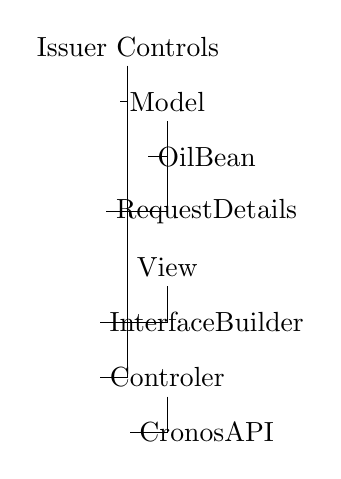
\begin{tikzpicture}[%
  grow via three points={one child at (0.5,-0.7) and
  two children at (0.5,-0.7) and (0.5,-1.4)},
  edge from parent path={(\tikzparentnode.south) |- (\tikzchildnode.west)}]
  \node {Issuer Controls}
    child { node {Model}
      child { node {OilBean}}
      child { node {RequestDetails}}
    }
    child [missing] {}				
    child [missing] {}		
    child { node {View}
    	child { node {InterfaceBuilder}}
    } 				
    child [missing] {}				
    child { node {Controler}
    	child
    	 {node {CronosAPI}}
    };
\end{tikzpicture}








\end{document}